
\section{Quantum Walk on a Line}
\label{sec:quantum_walk_line}

%proofed
Quantum Walk is the quantum version of random walks, which are mathematical formalisms that describe a path composed of random steps. A Markov Chain might be used to describe these processes.

We can define the Discrete Quantum Walk on a Line as a series of Left/Right decisions. Understanding this algorithm is important towards being able to define and design more complex algorithms that make use of quantum properties.

%proofed
 
%spelling 4; punctuation 3 weak

We followed an approach suggested by \cite{Ambainis} towards simulating n-steps of a Quantum Walk on a Line. The Matlab algorithm can be consulted on Appendix \ref{ap:a}.
In a discrete quantum walk in a line we want to preserve the fact that the probability of turning left is equal to the probability of turning right.  To represent a state in this algorithm we will need the number of the node and a direction (identified as L,R) \eqref{eq:3_qwl_state}.

%spelling 4; punctuation 3 weak

\begin{equation}
\label{eq:3_qwl_state}
\vert \psi\rangle = \vert n, L\rangle
\end{equation}

With two equally possible direction choices in each step, we can use a coin metaphor\cite{Ambainis}\cite{Ambainis2008} to approach the decision. We toss a coin and go either Left or Right depending on the result. 

In a quantum version we need to define a Coin Operator (Coin Matrix), which is responsible to imprint a direction to the current state. This operator is a unitary matrix in a 2-dimension Hilbert space. Some examples of Coin Operators are the Hadamard matrix\eqref{eq:hadamard} and a symmetric unitary matrix \eqref{eq:qwl_symmetric}.

\begin{equation}
\label{eq:hadamard}
H=\frac{1}{\sqrt{2}}\left[\begin{array}{cc}
1 & 1\\
1 & -1
\end{array}\right]
\end{equation}

\begin{equation}
\label{eq:qwl_symmetric}
\left[\begin{array}{cc}
\frac{1}{\sqrt{2}} & \frac{i}{\sqrt{2}}\\
\frac{i}{\sqrt{2}} & \frac{1}{\sqrt{2}}
\end{array}\right]
\end{equation}

Taking the Hadamard matrix as an example\eqref{eq:hadamard}, the coin matrix will operate on the state in the following way \eqref{eq:qwl_1}\eqref{eq:qwl_2}\cite{Ambainis}.

\begin{equation}
\label{eq:qwl_1}
C\vert n, L\rangle = \frac{1}{\sqrt{2}} \vert n, L\rangle + \frac{1}{\sqrt{2}} \vert n, R\rangle
\end{equation}
  
\begin{equation}
\label{eq:qwl_2}
C\vert n, R\rangle = \frac{1}{\sqrt{2}} \vert n, L\rangle - \frac{1}{\sqrt{2}} \vert n, R\rangle
\end{equation} 

The Coin Matrix obtains its name by being the quantum equivalent of flipping a classic coin. After tossing a coin comes an operator that will move the node in the direction assigned. The operator responsible for this modification is commonly referred as Shift Operator \eqref{eq:qwl_3}\eqref{eq:qwl_4}. 

\begin{equation}
\label{eq:qwl_3}
S\vert n, L\rangle = \frac{1}{\sqrt{2}} \vert n-1, L\rangle
\end{equation}

\begin{equation}
\label{eq:qwl_4}
S\vert n, R\rangle = \frac{1}{\sqrt{2}} \vert n+1, R\rangle
\end{equation} 

These matrices (Coin Matrix and Shift Operator) are used conceptually in various algorithms \cite{Rieffel2011}, therefore it is important to be familiar with them. A single step of the algorithm \ref{ap:a} is illustrated in Figure \ref{fig:qwl_tree}.

\begin{figure}[h]
\centering 

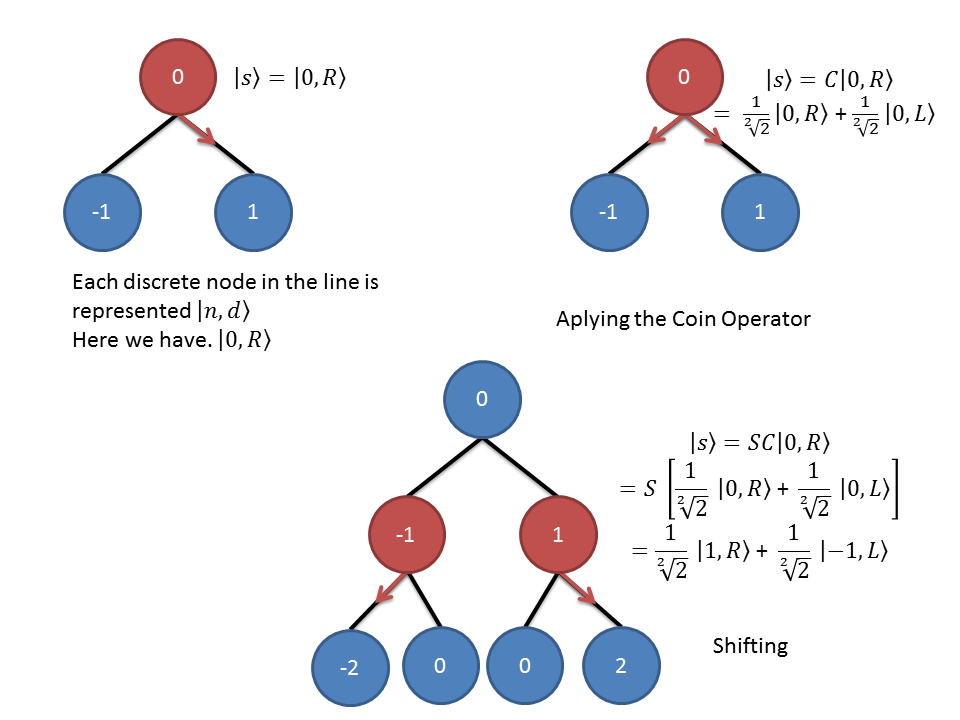
\includegraphics[scale=0.50]{Figures/quantum_walk_line.png}
\caption{Simulating a step of a discrete quantum walk on a line. In the beginning we have a state characterized by the position $(0)$ and a direction (either Left or Right).}
\label{fig:qwl_tree}
\end{figure}




\begin{figure}[h]
\centering 
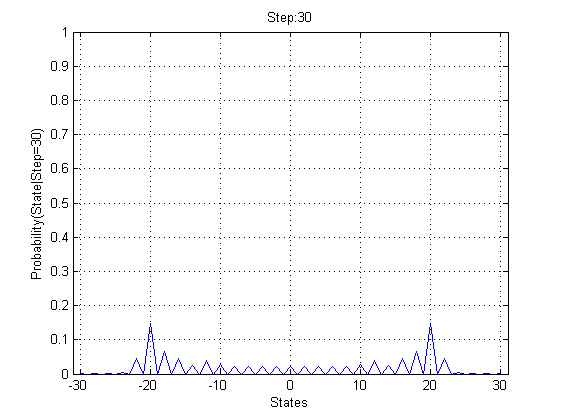
\includegraphics[scale=0.50]{Figures/quantum_walk_line_symetric.png}
\caption{30 Step of the Simulation \ref{ap:a} using Matrix \eqref{eq:hadamard} as a Coin Operator.}
\label{fig:qwl_symetric}
\end{figure}

\begin{figure}[h]
\centering 
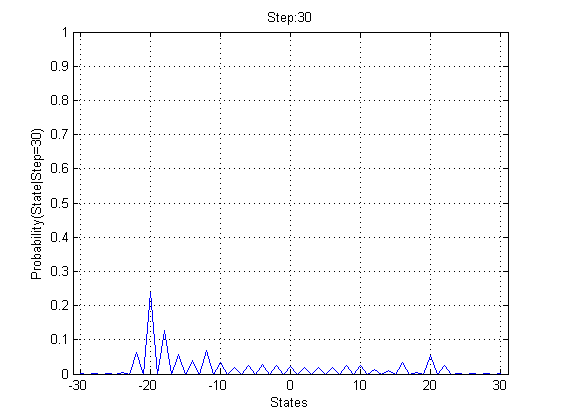
\includegraphics[scale=0.50]{Figures/quantum_walk_line_hadamard.png}
\caption{30 Step of the Simulation \ref{ap:a} using a Hadamard Matrix \eqref{eq:hadamard} as a Coin Operator.}
\label{fig:qwl_hadamard}
\end{figure}

If we took the classical approach in which we tossed a fair coin to decide to go either left or right, and after n-steps we measured the final node repeatedly, by the \ac{CLT} the final distribution would converge to a normal distribution. However, in the quantum approach, depending on the Coin Matrix we can get different distributions. In this simple problem we have the basis for some quantum algorithms. 

In Figures \ref{fig:qwl_hadamard} and \ref{fig:qwl_symetric}, depending on the coin operator we get two different results. Despite that, on one moment the  probability of shifting left, is always equal to the probability of shifting right. The main difference from the classical approach  lies on the fact there is a quantum interference during the walk, when we measure the results after $N$ steps, somewhat like the electrons interfere in the ``double-slit experiment'', presented in Section \ref{subsubsec:double_slit}. 


